\begin{surferIntroPage}{Superfici da record}{record_chmutovoktic}{Superfici da record del mondo}
Una superficie \`e detta \emph{non-singolare} o \emph{liscia} se non ha \emph{singularit\`a}, cio\`e se non ha punte o angoli. 
   La sfera e il toro sono esempi di superfici liscie, vedi le figure sotto.
   Se scegli una superficie in maniera casuale otterrai quasi sicuramente una liscia.  
 \begin{center}
      \vspace{-0.2cm}
      \begin{tabular}{@{}c@{}c@{}c@{\quad}c@{}c@{}c@{}c@{}}
        \begin{tabular}{@{}c@{}}
          liscia:
        \end{tabular}
        &
        \begin{tabular}{@{}c@{}}
          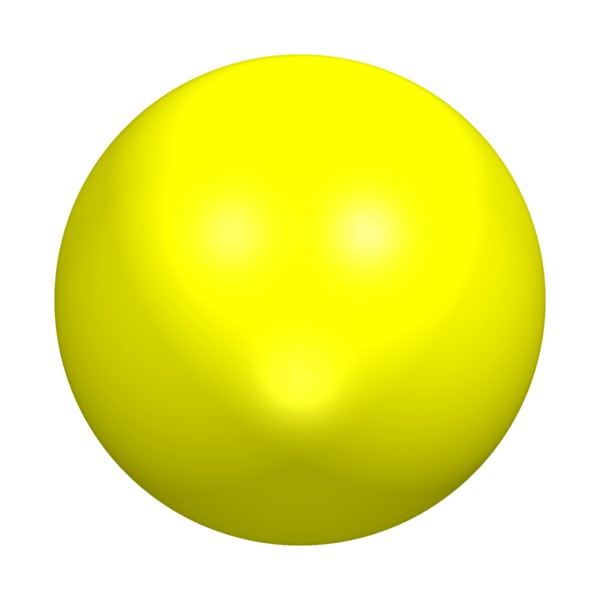
\includegraphics[width=1.1cm]{kugel}
        \end{tabular}
        &
        \begin{tabular}{@{}c@{}}
          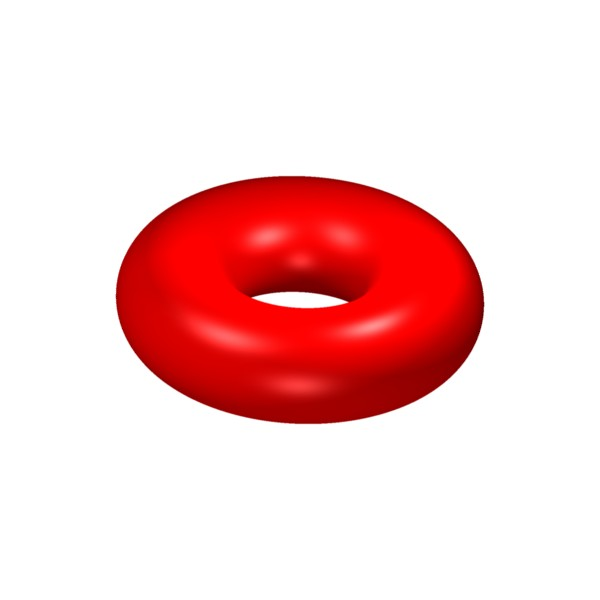
\includegraphics[width=1.1cm]{torus}
        \end{tabular}
        &
        \begin{tabular}{@{}c@{}}
          molte\\
          singolarit\`a:
        \end{tabular}
        &
        \begin{tabular}{c@{}@{}}
          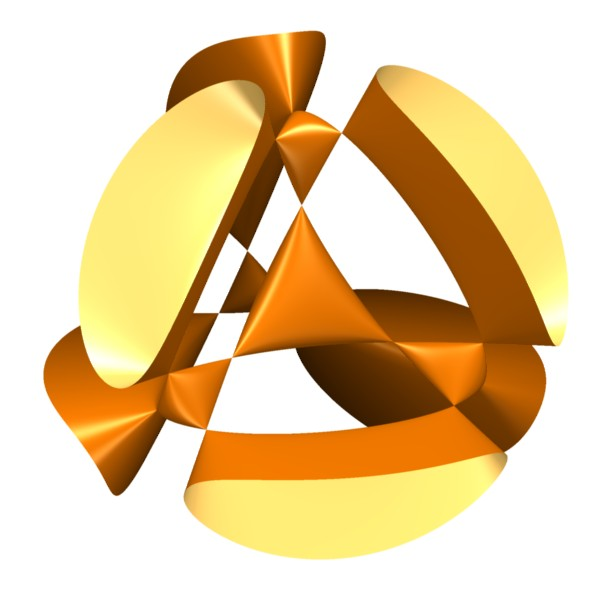
\includegraphics[width=1.1cm]{kummer}
        \end{tabular}
        &
        \begin{tabular}{c@{}@{}}
          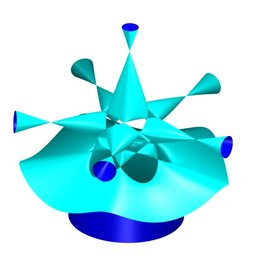
\includegraphics[width=1.1cm]{togliatti}
        \end{tabular}
        &
        \begin{tabular}{c@{}@{}}
          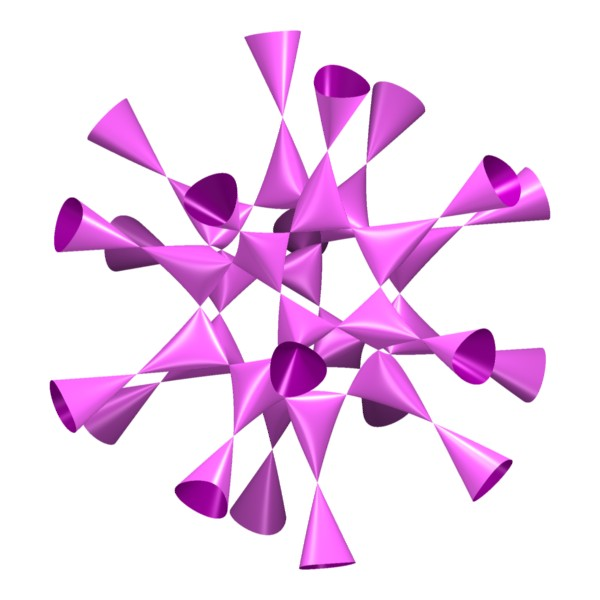
\includegraphics[width=1.1cm]{barth_sextic}
        \end{tabular}
      \end{tabular}
    \end{center}
    \vspace{-0.2cm}
   Solo superfici speciali hanno singolarit\`a. Per questo le singolarit\`a sono i punti pi\`u interessanti di una superficie.
    Le superfici nel programma SURFER sono definite da polinomi. Questo significa che le variabili nella formula appaiono con esponenti interi positivi. L'esponente pi\`u grande che appare nel polinomio si chiama \emph{grado} del polinomio. 
    Una domanda di ricerca matematica \`e quante singolarit\`a possa avere una superficie di un certo grado.
    Denotiamo questo numero con  $\mu(d)$, dove $d$ \`e il grado fissato.
  Questo numero \`e molto diffiicle da calcolare! Per gradi piccoli, $d=1,2,3,4$, \`e noto fin dal XIX secolo, ma per  $d=5$ \`e stato determinato solo nel 1980, e addirittura nel 1996 per $d=6$.
  E non si conosce ancora il numero massimo di singolarit\`a per una superficie di grado $d\ge 7$!   
  Sembra ancora molto lontano il momento in cui si potr\`a avere una risposta per ogni $d$.
  Ecco alcuni dei risultati ottenuti fino ad ora:
     
   \begin{center}
      \begin{tabular}{r|cccccccc|c}
        $d$ & $1$ & $2$ & $3$ & $4$ & $5$ & $6$ & $7$ & $8$ & $d$\\
        \hline
        \hline
        \rule{0pt}{1.2em}$\mu(d)\ge$ & $0$ & $1$ & $4$ & $16$ & $31$ & $65$ &
        $99$ & $168$ & 
        $\approx \frac{5}{12}d^3$\\[0.3em]
        \hline
        \rule{0pt}{1.2em}$\mu(d)\le$ & $0$ & $1$ & $4$ & $16$ & $31$ & $65$ &
        $104$ & $174$ & $\approx \frac{4}{9}d^3$
      \end{tabular}
    \end{center}
\end{surferIntroPage}
